\chapter{Ergebnis}

Im Kern besteht das Programm aus 3 Algorithmen.

\section{Randdetektion}

Das Bild wird Zeilenweise durchlaufen, bis ein Pixel gefunden wurde, der �ber dem Schwellwert f�r das Alpha liegt. Sobald ein entsprechender Pixel gefunden wurde, wird im Uhrzeigersinn nach einem Pixel gesucht, der Transparent ist und dessen rechter Nachbar im Alpha �ber dem Schwellwert liegt. Sobald der Start erreicht wird, ist der Pfad vervollst�ndigt und weitere Bilder werden gesucht.

\begin{figure}
	\centering
	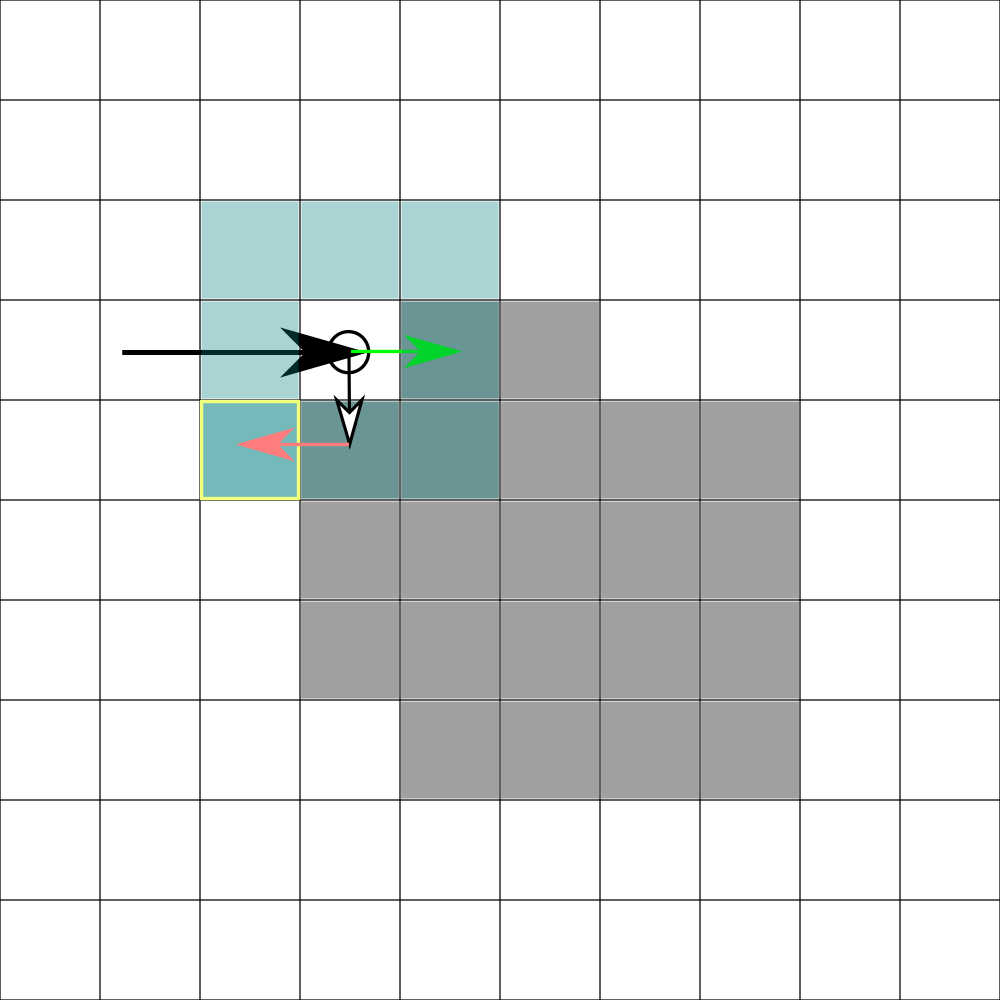
\includegraphics[width=0.33\textwidth]{images/RimDetection1.png}
	\caption{Rand Anfang }
	\label{fig1}
	Schwarzer Pfeil: Pixel Scan\\
	Gr�ner Pfeil: Pixel �ber Schwellwert\\
	Schwarz-wei�er Pfeil: Potenzieller Pfad\\
	Roter Pfeil: Rechts vom Potenziellen Pixel\\
	Gr�ne Felder: Punkte eines potenziellen Pfads\\
	Gr�nes Feld mit gelber Umrandung: Nachbar Scan
\end{figure}

\begin{figure}
	\centering
	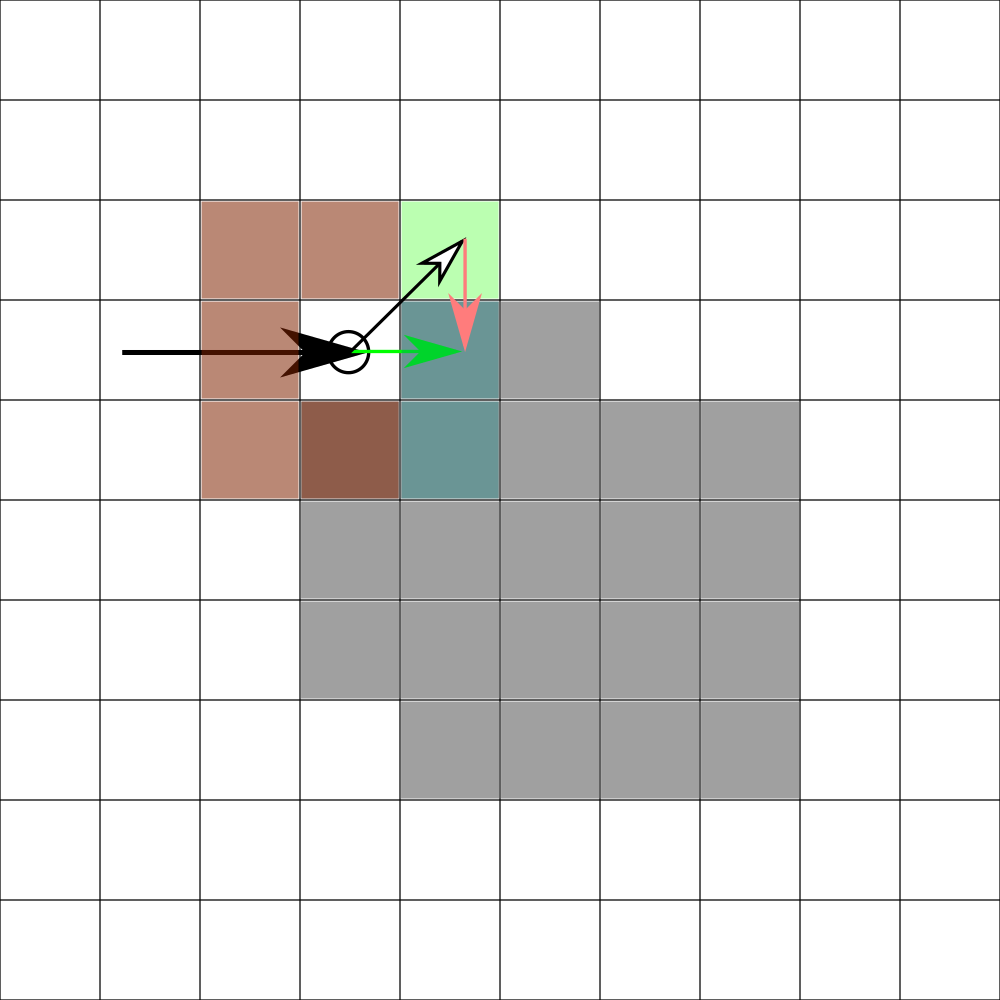
\includegraphics[width=0.33\textwidth]{images/RimDetection2.png}
	\caption{Gefundener n�chster Punkt }
	\label{fig2}
	Roter Felder: Ausgeschlossene Kandidaten \\
	Hellgr�nes Feld: Gefundener Rand
\end{figure}

\begin{figure}
	\centering
	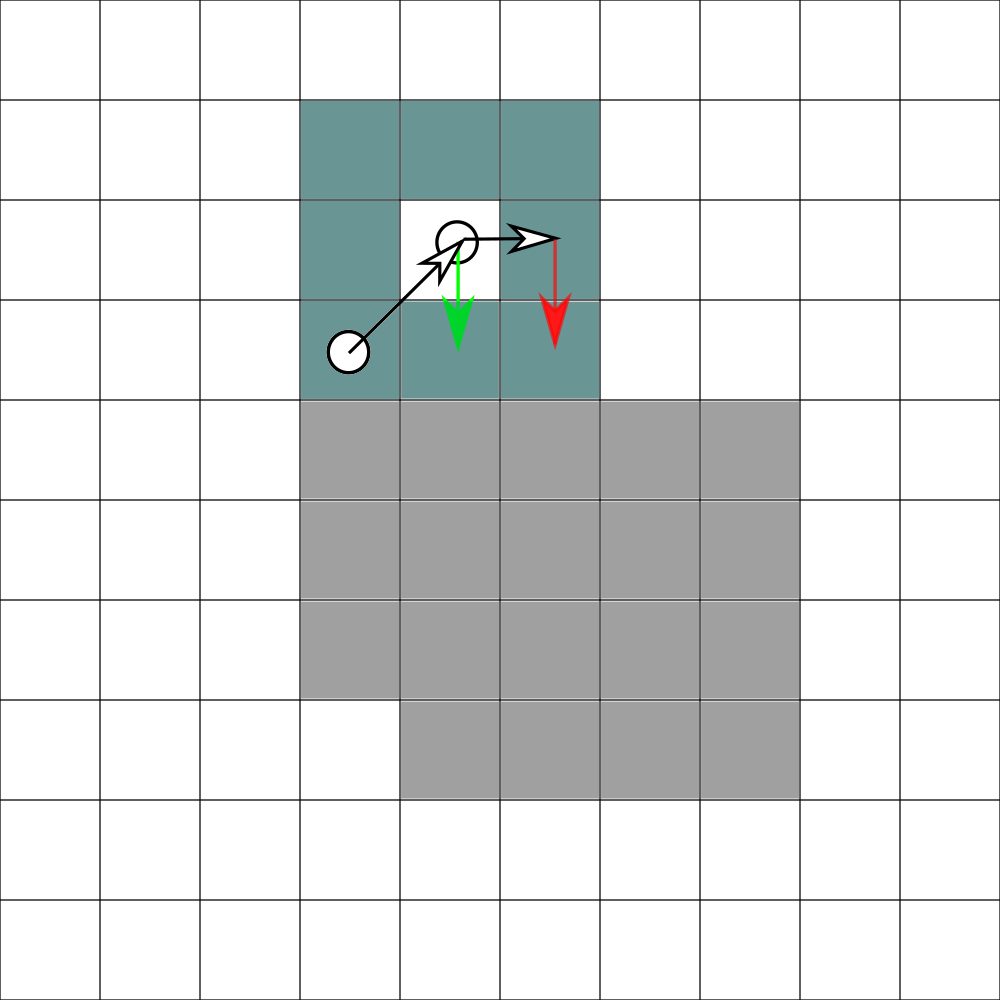
\includegraphics[width=0.33\textwidth]{images/RimDetection3.png}
	\caption{n�chster Punkt }
	\label{fig3}
\end{figure}

\begin{figure}
	\centering
	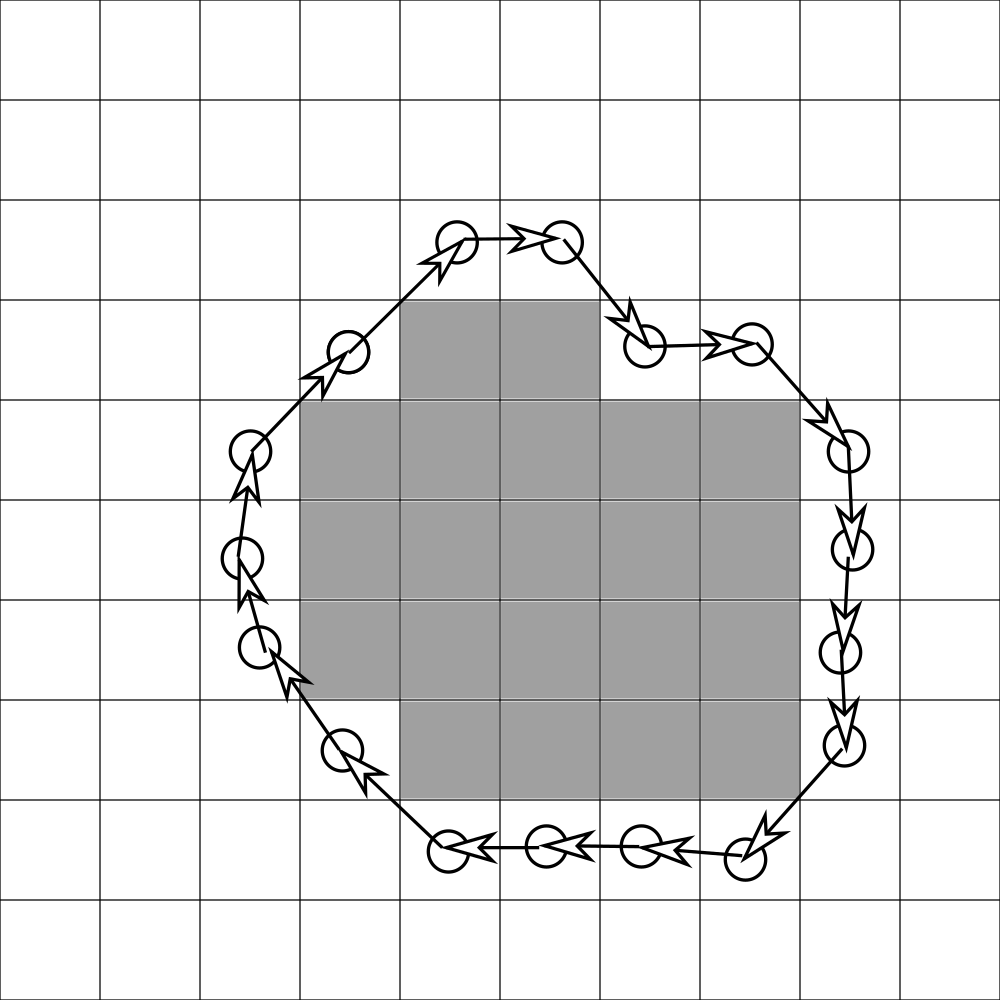
\includegraphics[width=0.33\textwidth]{images/RimDetection4.png}
	\caption{ Rand vollst�ndig }
	\label{fig4}
\end{figure}

\section{Ramer-Douglas-Peucker-Algorithmus}
Der Pfad besteht nun aus allen Pixeln, die den Rand darstellen. Da dies auch einige Geraden beinhaltet, l�sst sich der Rand gut vereinfachen, um sp�ter in der Triangulierung Dreiecke zu sparen.\\
Zur Vereinfachung wird der '"Ramer-Douglas-Peucker-Algorithmus'" verwendet. Dieser l�sst sich leicht implementieren und arbeitet zuverl�ssig.
\\
\\
Der Algorithmus sucht rekursiv den am weitesten entfernten Punkt zwischen Anfang und Ende. Wenn der Punkt von der Linie weiter als der Schwellwert entfernt ist, wird eine Spaltung der Linie durchgef�hrt. Wenn das Maximum innerhalb des Schwellwertes liegt, werden Anfangs- und Endpunkt direkt miteinander verbunden. \cite{Wikipedia:15}

\begin{figure}
	\centering
	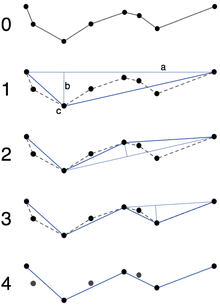
\includegraphics[width=0.33\textwidth]{images/220px-Douglas_Peucker.png}
	\caption{ Liniengl�ttung nach dem Douglas-Peucker-Algorithmus }
	\label{fig5}
\end{figure}

\newpage

\section{Ear clipping}
Ear clipping ist ein sehr einfach umzusetzender Triangulierungsalgorithmus von Polygonen.\\
Die Idee ist, jedes Ohr vom Polygon abzuschneiden, bis das ganze Polygon in einzelne Dreiecke zerlegt ist.
\cite{geometrictools:00}
\cite{delphigl:00}

\begin{figure}
	\centering
	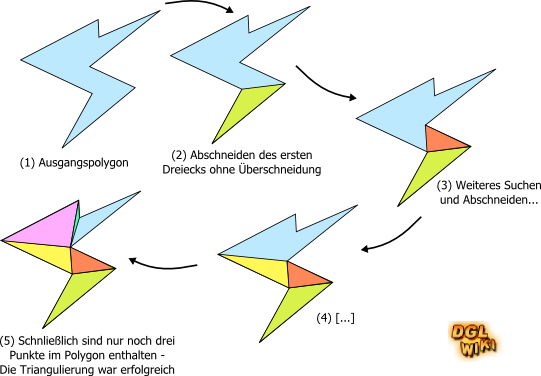
\includegraphics[width=1\textwidth]{images/Earclipping.png}
	\caption{ Ablauf des Ear Clipping Verfahrens }
	\label{fig6}
\end{figure}


